\documentclass[../main.tex]{subfiles}
\begin{document}

\section{Link Collision Avoidance  \\ \normalfont\normalsize\texttt{Emil Vincent Ancker}}
\label{sec:linkcollision}
The obstacle avoidance until now have only considered end-effector avoidance and since the robot is not just a point in Cartesian space, as considered until now, it is worth looking into link collision avoidance. In this section the robot under study is a redundant manipulator since the work is primarily based on \cite{maciejewski_obstacle_1985}, \cite{dae-hyung_park_movement_2008} and \cite{buss_introduction_nodate}. The chosen robot is a 7-DOF Franka Emika Panda which will be simulated in Matlab. An example of the robot and a spherical obstacle is shown in \autoref{fig:robot:vis}.
\begin{figure}[H]
    \centering
         \includegraphics[width=0.50\textwidth]{figures/robot_vis.png}
     \caption{Visualization of the robot and a spherical obstacle.}
     \label{fig:robot:vis}
\end{figure}

When performing link collision avoidance an additional repellent is needed to avoid the links of the robot colliding with an obstacle. But instead of incorporating this into the transformation system in \autoref{eq:system:transformation}, it is done through inverse kinematics \cite{dae-hyung_park_movement_2008}, making the end-effector follow the trajectory generated in previous sections while avoiding link collisions.\\

\subsection{Null Space Movement \\ \normalfont\normalsize\texttt{Emil Vincent Ancker}}
The end-effector velocity is related to the joint velocity through the Jacobian:
\begin{equation}
    \dot{\boldsymbol{x}}_e = \boldsymbol{J}_e \dot{\boldsymbol{q}}
\end{equation}
Where $\dot{\boldsymbol{x}}_e$ is the end-effector velocity and $\boldsymbol{J}_e$ is the Jacobian of the end-effector. Since the robot is a redundant manipulator the inverse of the Jacobian can not be found, instead the pseudoinverse is used to get a least-squares solution:
\begin{equation} \label{eq:link:iksol}
    \dot{\boldsymbol{q}} = \boldsymbol{J}_e^+ \dot{\boldsymbol{x}}_e
\end{equation}
Since the robot is a redundant manipulator this also means that there are more solutions to \autoref{eq:link:iksol}, this can be illustrated by introducing a null space movement \cite{maciejewski_obstacle_1985}:
\begin{equation} \label{eq:link:formula}
    \dot{\boldsymbol{q}} = \boldsymbol{J}_e^+\dot{\boldsymbol{x}}_e + \left( \boldsymbol{I} - \boldsymbol{J}_e^+\boldsymbol{J}_e \right)\boldsymbol{\mathcal{E}}
\end{equation}
The null space movement term in \autoref{eq:link:formula},
\begin{equation}
    \left( \boldsymbol{I} - \boldsymbol{J}_e^+\boldsymbol{J}_e \right)\boldsymbol{\mathcal{E}}
\end{equation}
Will map the arbitrary velocity, $\boldsymbol{\mathcal{E}}$, into the null space of $\boldsymbol{J}$ \cite{buss_introduction_nodate}. This means that we can now find a joint velocity corresponding to a Cartesian velocity and add an arbitrary joint movement that does not affect the Cartesian velocity.

\subsection{Utilizing Null Space Movement for Obstacle Avoidance \\ \normalfont\normalsize\texttt{Emil Vincent Ancker}}
The foundation of the utilization of null space movement to avoid obstacles builds on \autoref{eq:link:formula}, where the null space movement is adapted to avoid an obstacle \cite{dae-hyung_park_movement_2008}.

To incorporate the obstacle avoidance in the null space movement, the point on the robot $\boldsymbol{x}_0$ closest to the obstacle is considered,
\begin{equation} \label{eq:link:closest}
    \dot{\boldsymbol{x}}_0 = \boldsymbol{J}_0 \dot{\boldsymbol{q}}
\end{equation}
Where $\boldsymbol{J}_0$ is the Jacobian from the base up to $\boldsymbol{x}_0$. By imposing a constraint on the velocity of the robot closest to the obstacle, $\dot{\boldsymbol{x}}_0$, using a potential field it is possible to make this point, $\boldsymbol{x}_0$, move away from the obstacle. A potential field $U(\boldsymbol{x})$ is now considered \cite{dae-hyung_park_movement_2008}:
\begin{equation} \label{eq:link:pot}
    U(\boldsymbol{x}) = \begin{cases}
      \frac{\eta}{2}\left( \frac{1}{p(\boldsymbol{x})} - \frac{1}{p_0} \right)^2, & \text{if}\ p(\boldsymbol{x}) < p_0 \\
      0, & \text{otherwise}
    \end{cases}
\end{equation}
The potential field in \autoref{eq:link:pot} repels the point $\boldsymbol{x}$ away from the obstacle if it is within a threshold distance $p_0$. The term $p(\boldsymbol{x})$ is the distance from $\boldsymbol{x}$ to the obstacle. The repulsive effect is implemented by,
\begin{align} \label{eq:x0:velocity}
    \dot{\boldsymbol{x}}_0 &= - \gamma_{L} \nabla U(\boldsymbol{x}_0),\\
    \nabla_{\boldsymbol{x}} U(\boldsymbol{x}) &= \eta \left(\frac{1}{p(\boldsymbol{x})}-\frac{1}{p_0} \right)\left( \frac{-1}{p(\boldsymbol{x})^2}\right)\nabla_{\boldsymbol{x}}p(\boldsymbol{x})
\end{align}
Where $\gamma_{L}$ is a constant that has to be tuned. The derivative of the potential field is only as stated above when $p(\boldsymbol{x}) < p_0$.

By substituting \autoref{eq:link:formula} into \autoref{eq:link:closest}, the following is obtained:
\begin{equation}
    \dot{\boldsymbol{x}}_0 = \boldsymbol{J}_0 \left( \boldsymbol{J}_e^+\dot{\boldsymbol{x}}_e + \left( \boldsymbol{I} - \boldsymbol{J}_e^+\boldsymbol{J}_e \right)\boldsymbol{\mathcal{E}} \right)
\end{equation}
Since all entities in the above is known except the arbitrary velocity $\boldsymbol{\mathcal{E}}$, it can be isolated and the null-space velocity is obtained,
\begin{equation} \label{eq:link:nullspacevelocity}
    \boldsymbol{\mathcal{E}} = \left(\boldsymbol{J}_0(I-\boldsymbol{J}_e^+\boldsymbol{J}_e)\right)^+(\dot{\boldsymbol{x}}_0 - \boldsymbol{J}_0\boldsymbol{J}_e^+\dot{\boldsymbol{x}}_e)
\end{equation}
The expression for the null-space velocity, $\boldsymbol{\mathcal{E}}$, is now substituted into \autoref{eq:link:formula},
\begin{equation} \label{eq:readytosim}
    \dot{\boldsymbol{q}} = \boldsymbol{J}^+_e\dot{\boldsymbol{x}}_e + \left( \boldsymbol{I} - \boldsymbol{J}_e^+\boldsymbol{J}_e \right)\left(\boldsymbol{J}_0(I-\boldsymbol{J}_e^+\boldsymbol{J}_e)\right)^+(\dot{\boldsymbol{x}}_0 - \boldsymbol{J}_0\boldsymbol{J}_e^+\dot{\boldsymbol{x}}_e)
\end{equation}
According to \cite{maciejewski_obstacle_1985} \autoref{eq:readytosim} can be simplified to the following,
\begin{equation} \label{eq:link:final}
        \dot{\boldsymbol{q}} = \boldsymbol{J}^+_e\dot{\boldsymbol{x}}_e +\left(\boldsymbol{J}_0(I-\boldsymbol{J}_e^+\boldsymbol{J}_e)\right)^+(\dot{\boldsymbol{x}}_0 - \boldsymbol{J}_0\boldsymbol{J}_e^+\dot{\boldsymbol{x}}_e)
\end{equation}
Everything is now known and therefore the link collision avoidance can now be implemented.

\subsection{Implementation of Pseudoinverse based Link Collision Avoidance   \\ \normalfont\normalsize\texttt{Emil Vincent Ancker}}
In \autoref{eq:link:final} it is necessary to find the closest point $\boldsymbol{x}_0$ to determine both $\boldsymbol{J}_0$ and $\dot{\boldsymbol{x}}_0$. It was chosen to discretize the robot into 7 points located at each joint, which can be seen in \autoref{fig:link:points}.
\begin{figure}[H]
    \centering
    \begin{subfigure}[b]{0.48\textwidth}
        \centering
        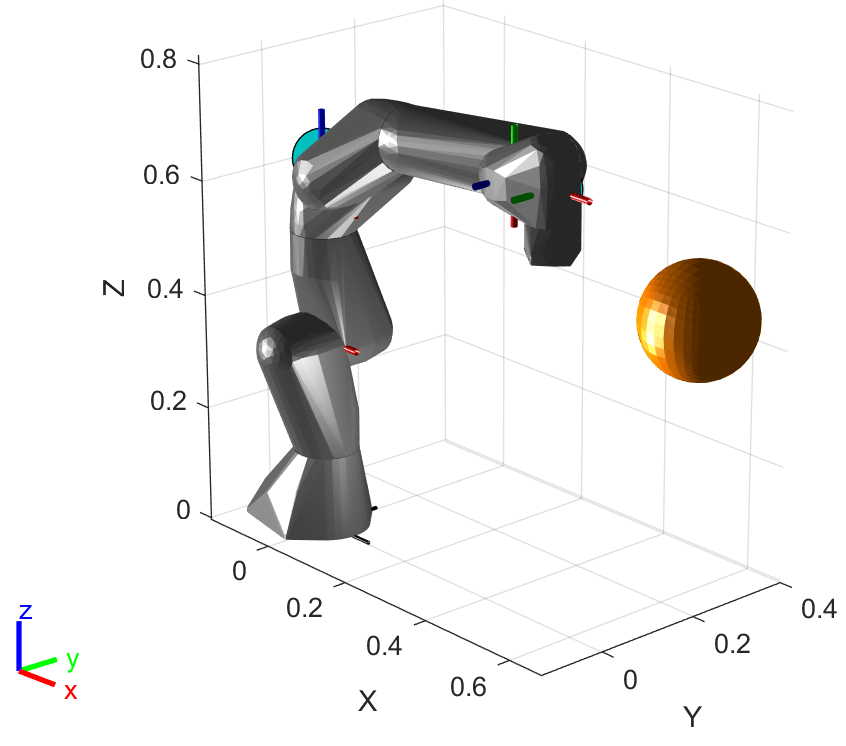
\includegraphics[width=\textwidth]{figures/linkcollision/robot_points_vis.png}
        \caption{Robot with body meshes shown and indication of points.}
        \label{fig:link:points:withmesh}
    \end{subfigure}
    \hfill
    \begin{subfigure}[b]{0.48\textwidth}
        \centering
        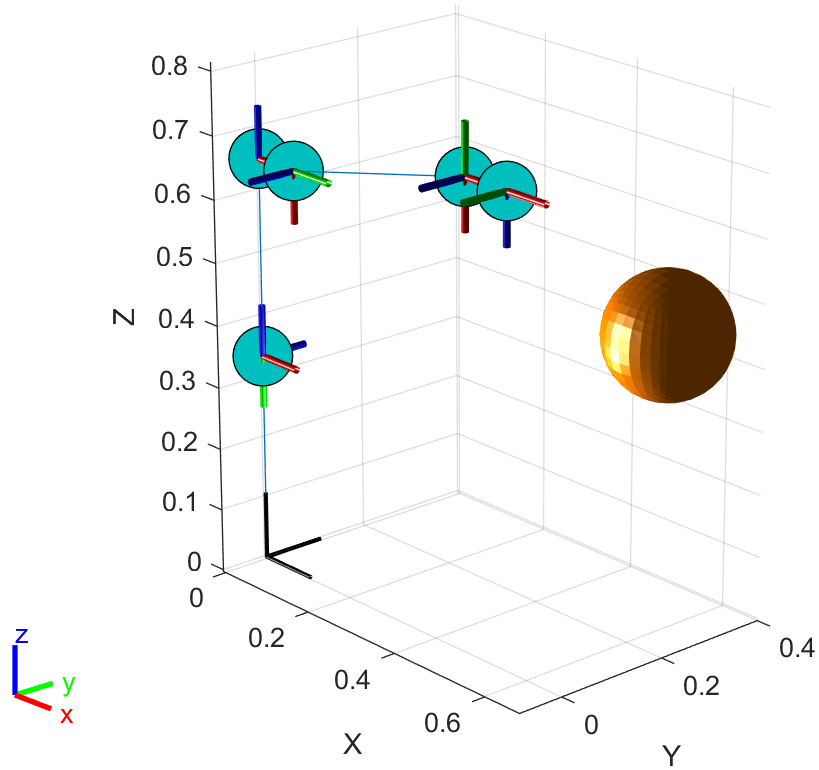
\includegraphics[width=\textwidth]{figures/linkcollision/robot_points_vis_no_mesh.png}
        \caption{Robot without body meshes shown and indication of points.}
        \label{fig:link:points:nomesh}
    \end{subfigure}
    \caption{Robot shown with and without body meshes and with indication of points to show where the points that are being observed are located on the robot.}
    \label{fig:link:points}
\end{figure}
The point $\boldsymbol{x}_0$ is set to the point on the robot which is closest to the obstacle.
The procedure at each time step for the link collision avoidance is shown in \autoref{alg:avoidance}, the trajectory given as input $\boldsymbol{T}$ might change while the robot is evaluating according to the online obstacle avoidance in \autoref{subsec:avoidance:online}.\\
\begin{algorithm}[H]
 \SetAlgoLined
 \textbf{Requires initialization of: }$\boldsymbol{T}$\text{ (trajectory)}, $\Delta t$\text{ (time step)}, $\boldsymbol{q}$\text{ (initial configuration)}.\\
 \While{\text{points left in $\boldsymbol{T}$}}{
    \nl $\dot{\boldsymbol{x}}_e = \frac{\boldsymbol{T}_{i+1} - \boldsymbol{T}_i}{\Delta t}$ \\
    \nl $\boldsymbol{x}_0 = \underset{\boldsymbol{x}}{\text{arg min }}||(\boldsymbol{o} - \boldsymbol{x}_{i})||^2$ \Comment{find point on robot closest to obstacle}\\
    \nl $\dot{\boldsymbol{x}}_0 = -\gamma_L \nabla U(\boldsymbol{x}_0) $ \\
    \nl $\boldsymbol{J}_0 = \text{ComputeJacobian}(\boldsymbol{x}_0)$ \\
    \nl $\boldsymbol{J}_e = \text{ComputeJacobian}(\boldsymbol{x}_e)$ \\
    \nl $\dot{\boldsymbol{q}} = \boldsymbol{J}^+_e\dot{\boldsymbol{x}}_e +\left(\boldsymbol{J}_0(I-\boldsymbol{J}_e^+\boldsymbol{J}_e)\right)^+(\dot{\boldsymbol{x}}_0 - \boldsymbol{J}_0\boldsymbol{J}_e^+\dot{\boldsymbol{x}}_e)$ \\
    \nl $\boldsymbol{q} = \boldsymbol{q} + \dot{\boldsymbol{q}} \Delta t$ \Comment{configuration is being updated}
 }
 \caption{Link collision avoidance}
 \label{alg:avoidance}
\end{algorithm}
By using the computed joint velocities in \autoref{alg:avoidance} which is based on \cite{maciejewski_obstacle_1985} and \cite{dae-hyung_park_movement_2008} multiple problems were observed.\\

The first problem observed was that the term $(J_0(I - J_e^+ J_e))^+$ often becomes singular or close to, which produces very high joint velocities, this problem could simply be avoided by introducing thresholding on the Moore-Penrose inverse. Another problem was observed, but this was with respect to the term $\boldsymbol{J}^+_e\dot{\boldsymbol{x}}_e$, which produces very high joint velocities when the robot is close to a singularity.\\
The problems can be illustrated by giving the trajectory generated by the DMP as input, and inspecting the joint velocities for the third joint from the base shown in \autoref{fig:link:problem:joint3}.

\begin{figure}[H]
    \centering
    \begin{subfigure}[b]{0.48\textwidth}
        \centering
        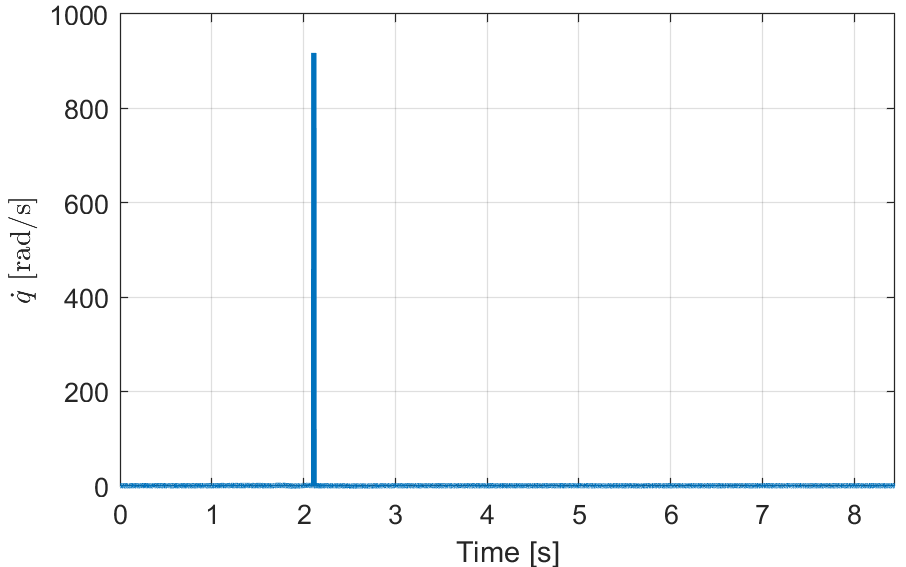
\includegraphics[width=\textwidth]{figures/linkcollision/joint_3_vel_1.png}
        \caption{Joint velocities for the third joint directly obtained from the inverse kinematics solution.}
        \label{fig:link:problem:joint3:1}
    \end{subfigure}
    \hfill
    \begin{subfigure}[b]{0.48\textwidth}
        \centering
        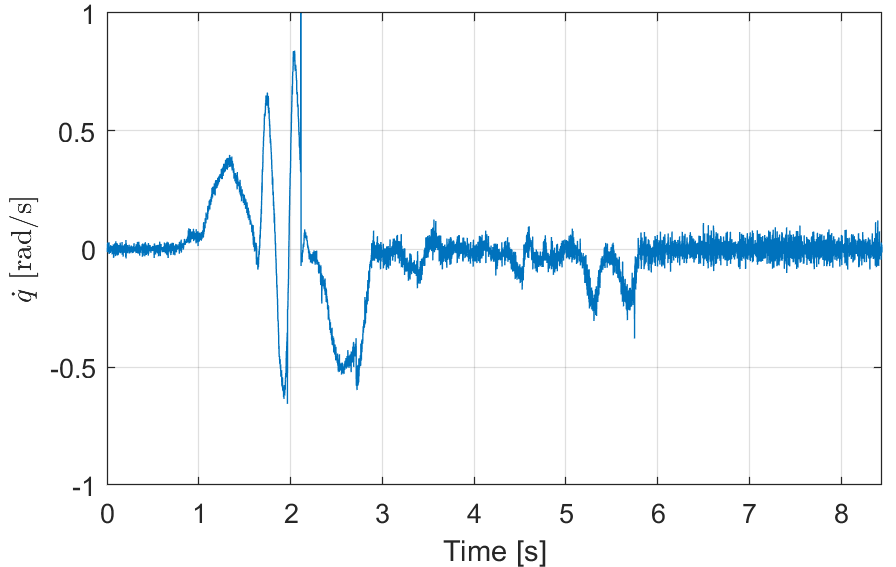
\includegraphics[width=\textwidth]{figures/linkcollision/joint_3_vel_2.png}
        \caption{Joint velocities for the third joint with limits on the y-axis of $[-1,\ 1]$.}
        \label{fig:link:problem:joint3:2}
    \end{subfigure}
    \caption{Joint velocities obtained from inverse kinematics with null space movement.}
    \label{fig:link:problem:joint3}
\end{figure}
In \autoref{fig:link:problem:joint3:1} it can be observed that approximately two seconds into the execution of the trajectory, the inverse kinematics leads to joint velocity of infeasibly large magnitude. The resulting trajectory can be seen in \autoref{fig:link:problem:xe}.
\begin{figure}[H]
    \centering
         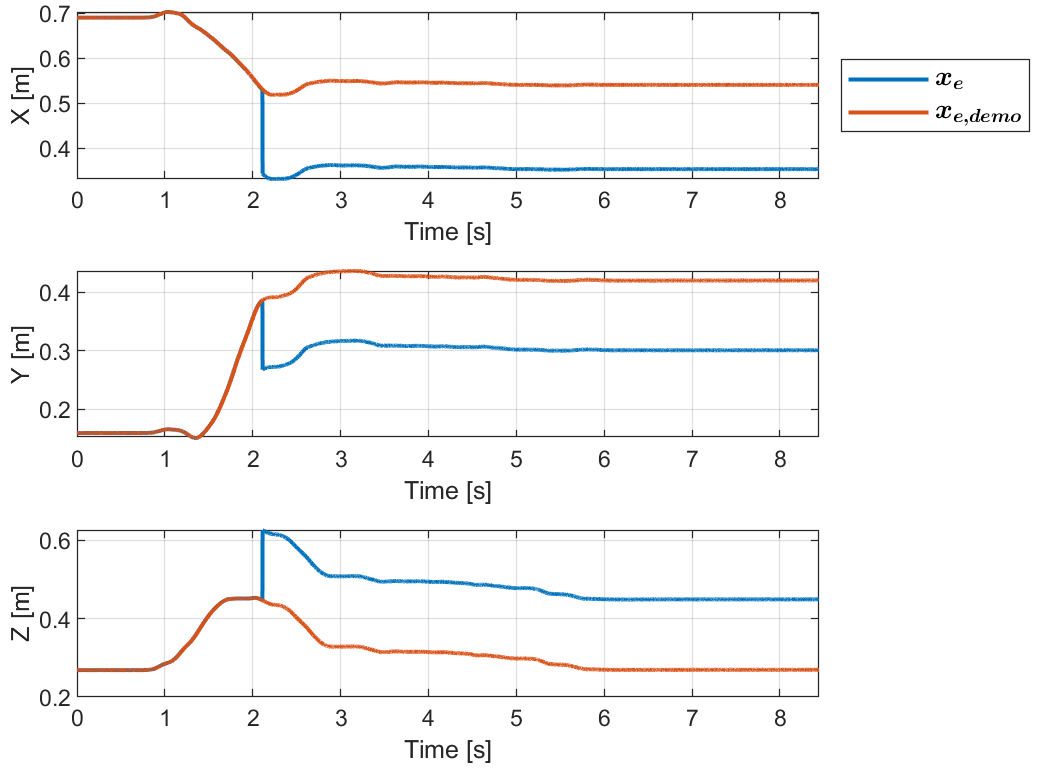
\includegraphics[width=0.85\textwidth]{figures/linkcollision/inversekin_prob_xe.png}
     \caption{Resulting trajectory from the generated joint velocities from inverse kinematics based on pseudoinverse Jacobian.}
     \label{fig:link:problem:xe}
\end{figure}
The problem of inverse kinematics based on pseudoinverse observed in \autoref{fig:link:problem:joint3} and \autoref{fig:link:problem:xe} is also stated in \cite{buss_introduction_nodate}, where damped least squares for inverse kinematics is suggested to handle configurations close to singularities better.

\subsection{Damped Least Squares for Inverse Kinematics   \\ \normalfont\normalsize\texttt{Emil Vincent Ancker}}
The inverse kinematics problem is stated as a minimization problem, where the objective is to minimize the error $\boldsymbol{J}\dot{\boldsymbol{q}} - \dot{\boldsymbol{x}_e}$ and punish the solution by the magnitude of $\dot{\boldsymbol{q}}$. The minimization problem is as follows \cite{buss_introduction_nodate},
\begin{equation} \label{eq:inverse:min}
    \text{min } f(\dot{\boldsymbol{q}}) = ||\boldsymbol{J}\dot{\boldsymbol{q}} - \dot{\boldsymbol{x}_e}||^2 + \lambda^2||\dot{\boldsymbol{q}}||^2
\end{equation}
Where $\lambda \in \mathbb{R}$ is a non-zero damping constant \cite{buss_introduction_nodate}. The solution minimizing the problem in \autoref{eq:inverse:min} is as follows \cite{buss_introduction_nodate},
\begin{equation} \label{eq:damped:withinv}
    \dot{\boldsymbol{q}} = \boldsymbol{J}^T(\boldsymbol{J}\boldsymbol{J}^T + \lambda^2\boldsymbol{I})^{-1}\dot{\boldsymbol{x}}_e
\end{equation}
The solution in \autoref{eq:damped:withinv} can also be found by formulating the solution as a system of linear equations,
\begin{equation} \label{eq:damped:linsys}
    (\boldsymbol{J}_e \boldsymbol{J}_e^T + \lambda^2 \boldsymbol{I})\boldsymbol{f} = \dot{\boldsymbol{x}}_e
\end{equation}
Once the solution to the linear system in \autoref{eq:damped:linsys} have been found the joint velocities can be found,
\begin{equation} \label{eq:damped:semisol}
    \dot{\boldsymbol{q}} = \boldsymbol{J}_e^T \boldsymbol{f}
\end{equation}
Finally, the null space movement is added to the found joint velocity in \autoref{eq:damped:semisol} to enable link collision avoidance,
\begin{equation} \label{eq:damped:solution}
    \dot{\boldsymbol{q}} = \boldsymbol{J}_e^T \boldsymbol{f} +\left(\boldsymbol{J}_0(I-\boldsymbol{J}_e^+\boldsymbol{J}_e)\right)^+(\dot{\boldsymbol{x}}_0 - \boldsymbol{J}_0\boldsymbol{J}_e^+\dot{\boldsymbol{x}}_e)
\end{equation}
By following the same trajectory as done for the pseudoinverse based inverse kinematics it results in the trajectory shown in \autoref{fig:link:damped:problem}.
\begin{figure}[H]
    \centering
         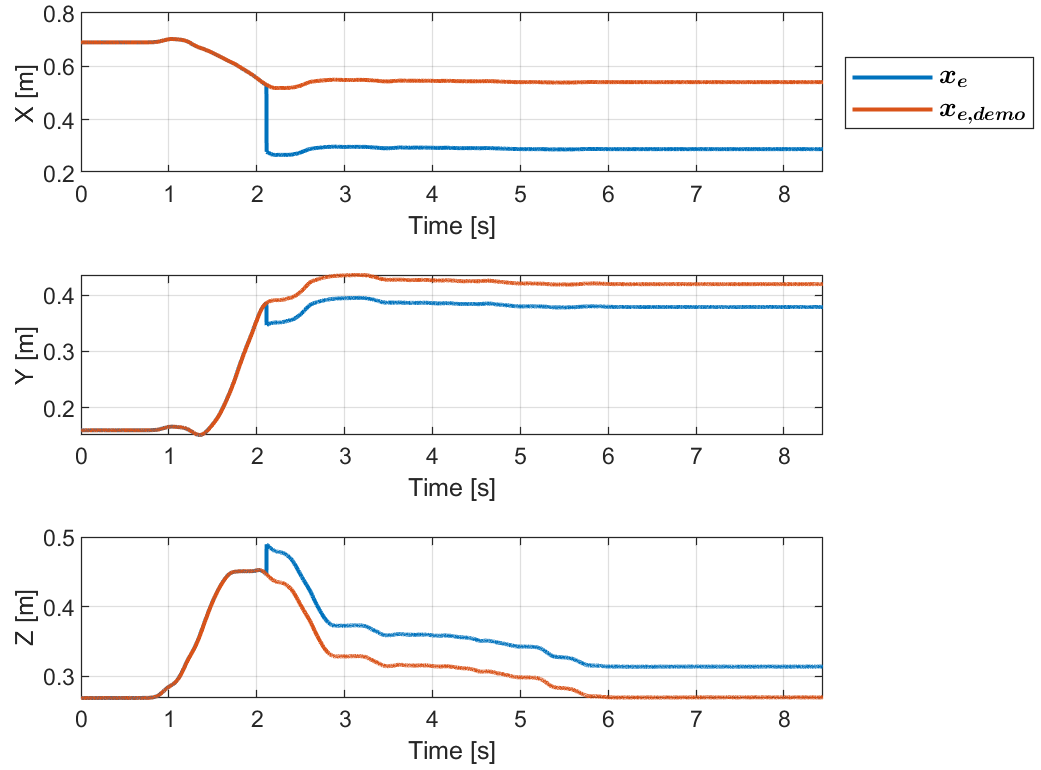
\includegraphics[width=0.85\textwidth]{figures/linkcollision/inversekin_damped_problem.png}
     \caption{Resulting trajectory from the generated joint velocities from inverse kinematics based on damped least squares. With damping coefficient $\lambda = 0.05$.}
     \label{fig:link:damped:problem}
\end{figure}
It can be seen from the generated trajectory, that the solution found by \autoref{eq:damped:solution} is less sensitive to singularities, but it does still have an impact on the path.

\subsubsection{Attracting the End-effector   \\ \normalfont\normalsize\texttt{Emil Vincent Ancker}}
Instead of using the end-effector velocity generated from the DMPs, $\dot{\boldsymbol{x}}_{DMP}$, directly a trajectory error is defined,
\begin{equation}
    \dot{\boldsymbol{x}}_{e} = \frac{\boldsymbol{x}_{e,demo} - \boldsymbol{x}_e}{dt}, \quad dt = \frac{1}{500}
\end{equation}
By directly introducing this into the solution, the response in \autoref{fig:link:damped:problem} is obtained.
\begin{figure}[H]
    \centering
         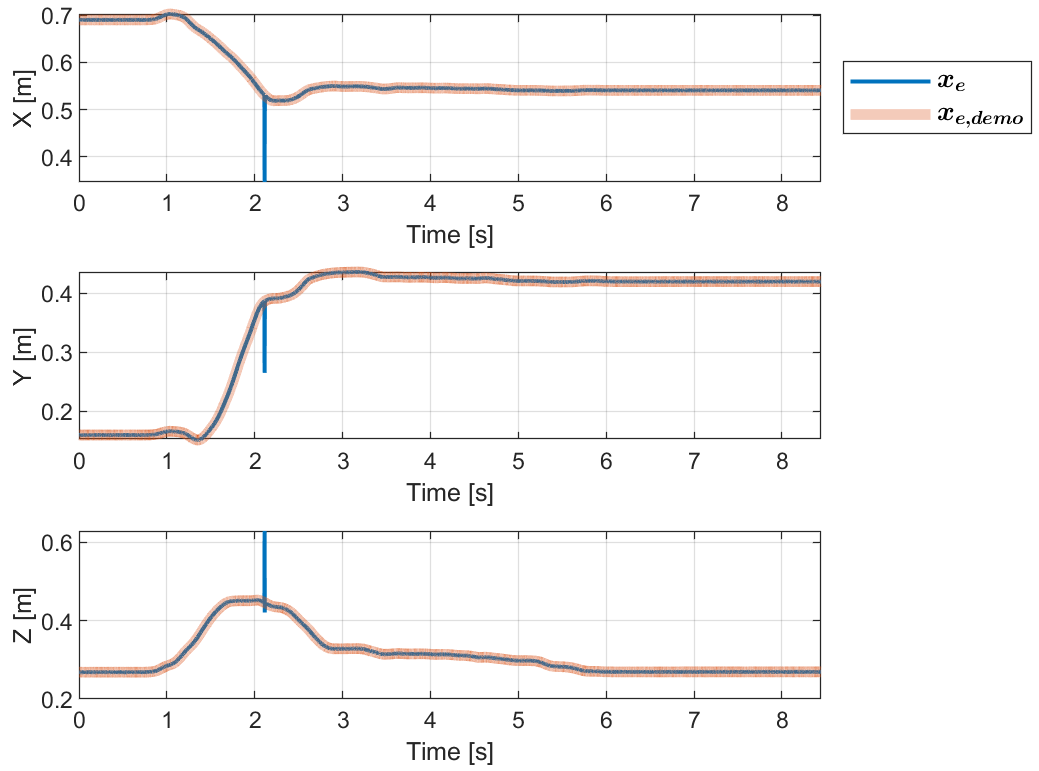
\includegraphics[width=0.85\textwidth]{figures/linkcollision/inversekin_damped_ok.png}
     \caption{Resulting trajectory from the generated joint velocities from inverse kinematics based on damped least squares while taking current end-effector position into account. With damping coefficient $\lambda = 0.05$.}
     \label{fig:link:damped:ok}
\end{figure}
The resulting joint velocity is still infeasibly high, and might be improved by using \texttt{ClampAbsMax}, which is shown in \autoref{eq:link:clamp}.
\begin{equation} \label{eq:link:clamp}
    \text{ClampAbsMax}(\dot{\boldsymbol{q}} , d) =  \begin{cases}
      \dot{\boldsymbol{q}}, & ||\dot{\boldsymbol{q}}|| < d \\
      d \frac{\dot{\boldsymbol{q}}}{||\dot{\boldsymbol{q}}||}, & \text{otherwise}
    \end{cases}
\end{equation}
By utilizing ClampAbsMax the resulting path in \autoref{fig:link:damped:good} is obtained.
\begin{figure}[H]
    \centering
         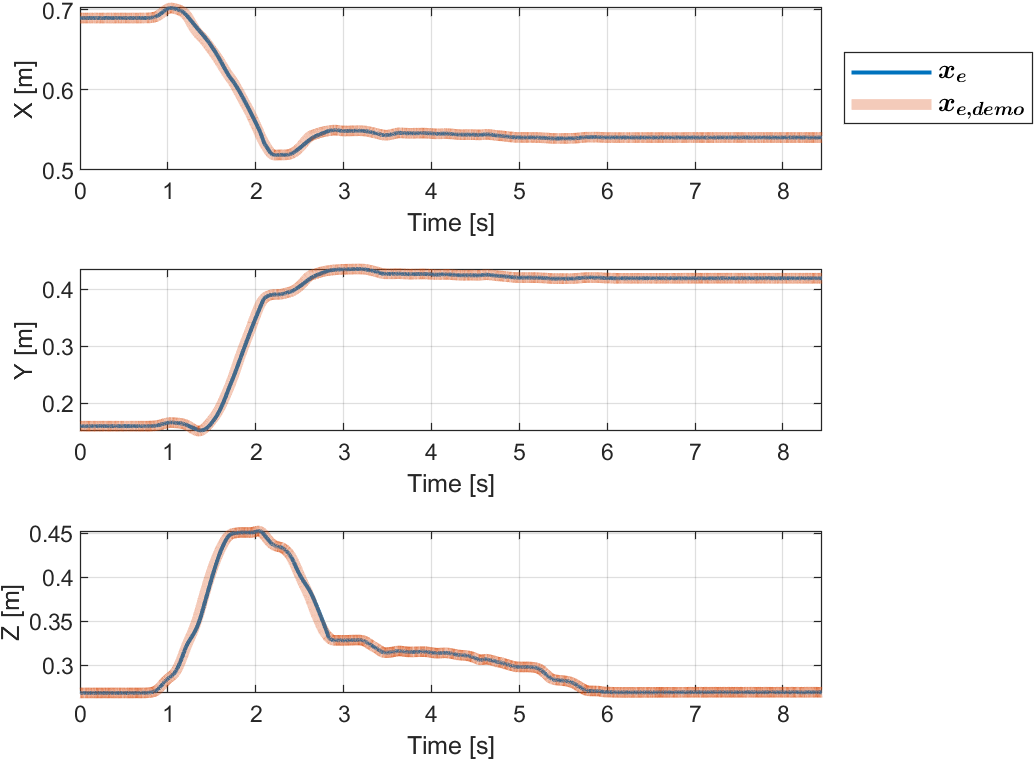
\includegraphics[width=0.85\textwidth]{figures/linkcollision/inversekin_damped_good.png}
     \caption{Resulting trajectory from the generated joint velocities from inverse kinematics based on damped least squares while taking current end-effector position into account and utilizing ClampAbsMax with $d = 1 [rad/s]$ and damping coefficient $\lambda = 0.05$.}
     \label{fig:link:damped:good}
\end{figure}
An example of the joint velocities is shown in \autoref{fig:link:damped:good:joint}, where the joint velocities for the third joint is shown.
\begin{figure}[H]
    \centering
         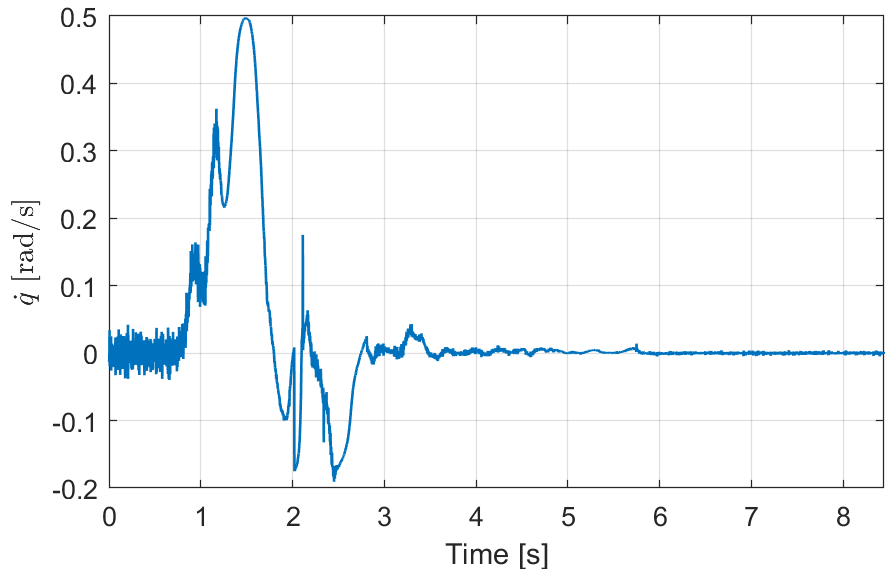
\includegraphics[width=0.65\textwidth]{figures/linkcollision/joint_3_vel_damped_good.png}
     \caption{Resulting joint velocity for the third joint from inverse kinematics based on damped least squares while taking current end-effector position into account and utilizing ClampAbsMax with $d = 1 [rad/s]$ and damping coefficient $\lambda = 0.05$.}
     \label{fig:link:damped:good:joint}
\end{figure}

\subsubsection{Introducing an Obstacle}
By setting the strength of the potential field to $\gamma_L = 1.0$ and introducing an obstacle at location $\boldsymbol{o} = (0.25,\ 0.25,\ 0.45)^T$ the response in \autoref{fig:link:damped:obstacle}.
\begin{figure}[H]
    \centering
         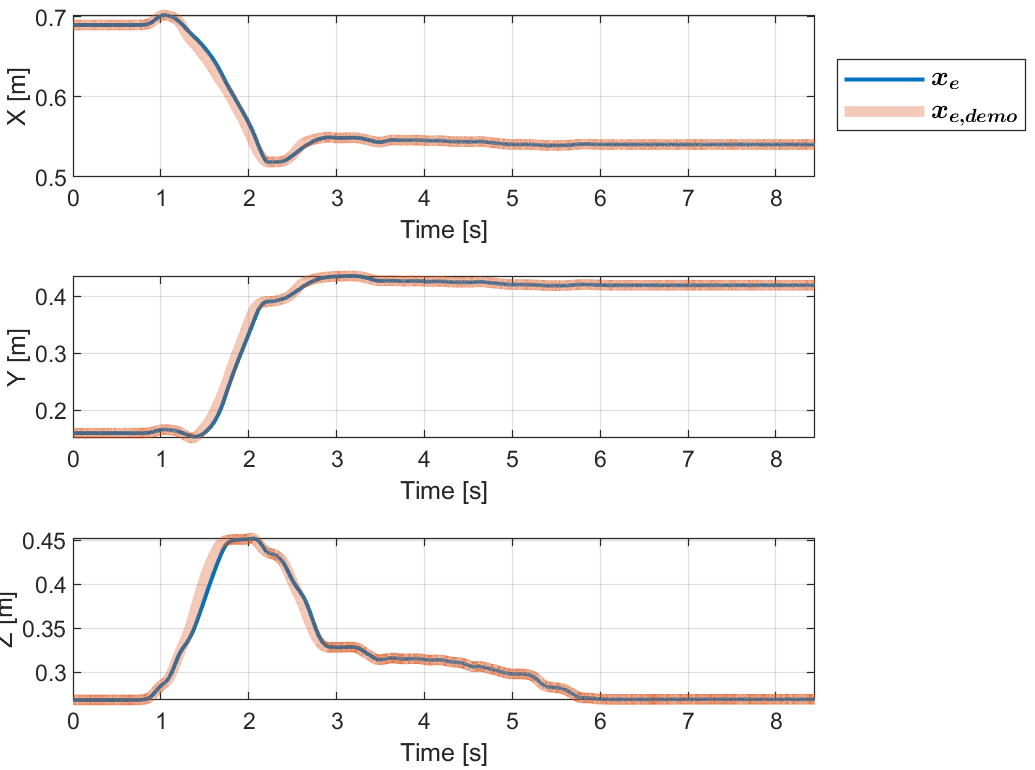
\includegraphics[width=0.85\textwidth]{figures/linkcollision/DLS_gamma1.png}
     \caption{Link collision avoidance performed using inverse kinematics based on damped least squares utilizing ClampAbsMax with $d = 1 [rad/s]$, damping coefficient $\lambda = 0.05$ and potential field strength $\gamma_L = 1.0$.}
     \label{fig:link:damped:obstacle}
\end{figure}
It can be seen in \autoref{fig:link:damped:obstacle} that there is a negligible small deviation from the path. Visualization of a link collision can be seen in \autoref{fig:link:example:collision}, while a link collision avoidance can be seen in \autoref{fig:link:example:collisionavoidance}. Animations showing multiple examples of link collision and link collision avoidance are available on the project's Github repository\footnote{\url{https://github.com/Masle16/obstacle_avoidance_with_dmps/tree/master/LinkCollisionAvoidance/GIF}}. 
\begin{figure}[H]
    \centering
    \begin{subfigure}[b]{0.24\textwidth}
        \centering
        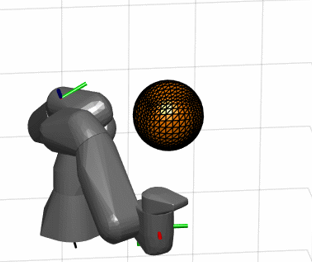
\includegraphics[width=\textwidth]{figures/linkcollision/g0_1.png}
        \label{}
    \end{subfigure}
    \begin{subfigure}[b]{0.24\textwidth}
        \centering
         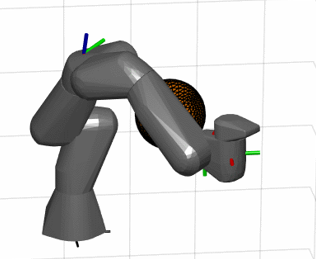
\includegraphics[width=\textwidth]{figures/linkcollision/g0_2.png}
        \label{}
    \end{subfigure}
    \hfill
    \begin{subfigure}[b]{0.24\textwidth}
        \centering
         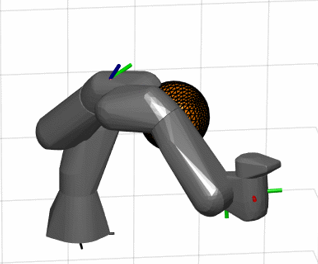
\includegraphics[width=\textwidth]{figures/linkcollision/g0_3.png}
        \label{}
    \end{subfigure}
    \hfill
    \begin{subfigure}[b]{0.24\textwidth}
        \centering
         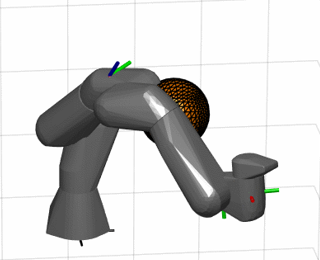
\includegraphics[width=\textwidth]{figures/linkcollision/g0_4.png}
        \label{}
    \end{subfigure}
    \caption{Example of a link collision. Strength of potential field is set to $\gamma_L = 0$.}
    \label{fig:link:example:collision}
\end{figure}

\begin{figure}[H]
    \centering
    \begin{subfigure}[b]{0.24\textwidth}
        \centering
        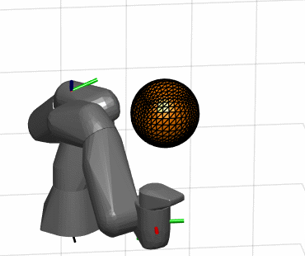
\includegraphics[width=\textwidth]{figures/linkcollision/g100_1.png}
        \label{}
    \end{subfigure}
    \begin{subfigure}[b]{0.24\textwidth}
        \centering
         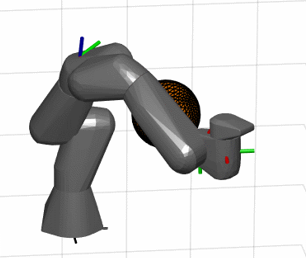
\includegraphics[width=\textwidth]{figures/linkcollision/g100_2.png}
        \label{}
    \end{subfigure}
    \hfill
    \begin{subfigure}[b]{0.24\textwidth}
        \centering
         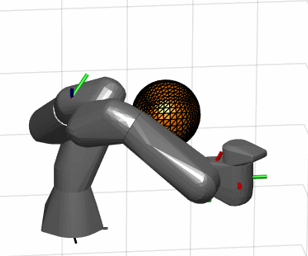
\includegraphics[width=\textwidth]{figures/linkcollision/g100_3.png}
        \label{}
    \end{subfigure}
    \hfill
    \begin{subfigure}[b]{0.24\textwidth}
        \centering
         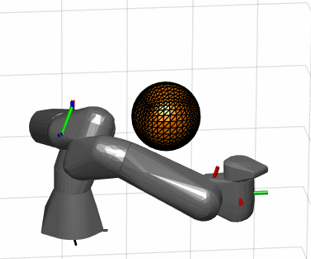
\includegraphics[width=\textwidth]{figures/linkcollision/g100_4.png}
        \label{}
    \end{subfigure}
    \caption{Example of link collision avoidance. Strength of potential field is set to $\gamma_L = 100$.}
    \label{fig:link:example:collisionavoidance}
\end{figure}

An example of the resulting joint velocities is once again shown for the third joint in \autoref{fig:link:damped:obstacle:joint}, where it clearly can be seen that the joint has a new velocity profile to incorporate the link collision avoidance.
\begin{figure}[H]
    \centering
         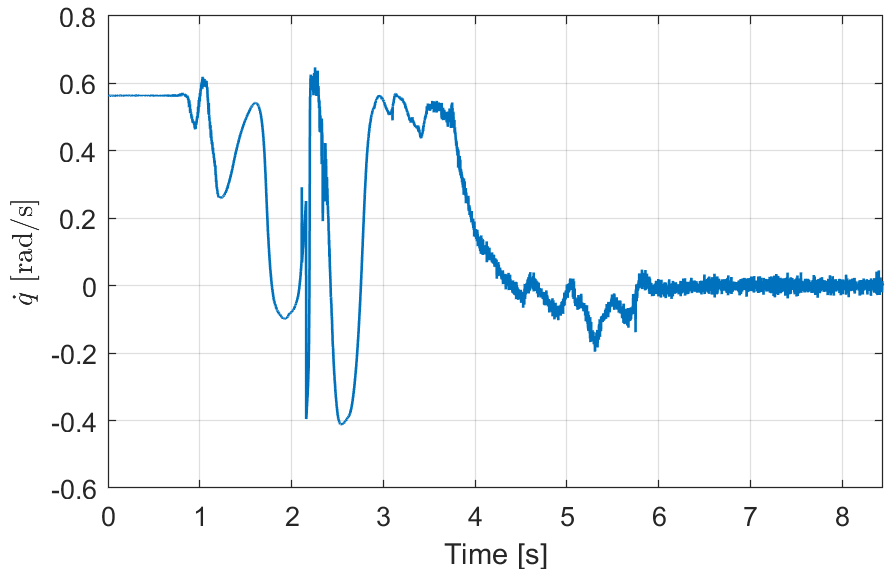
\includegraphics[width=0.65\textwidth]{figures/linkcollision/joint_3_vel_obstacle.png}
     \caption{Resulting joint velocity for the third joint when performing link collision avoidance using inverse kinematics based on damped least squares while taking current end-effector position into account and utilizing ClampAbsMax with $d = 1 [rad/s]$, damping coefficient $\lambda = 0.05$ and potential field strength $\gamma_L = 1.0$.}
     \label{fig:link:damped:obstacle:joint}
\end{figure}
The final procedure at each time step when performing link collision avoidance is shown in \autoref{alg:damped:avoidance}.\\
\begin{algorithm}[H]
 \SetAlgoLined
 \textbf{Requires initialization of: }$\boldsymbol{T}$\text{ (trajectory)}, $\Delta t$\text{ (time step)}, $\boldsymbol{q}$\text{ (initial configuration)}.\\
 \While{\text{points left in $\boldsymbol{T}$}}{
    \nl $\dot{\boldsymbol{x}}_e = \frac{\boldsymbol{T}_{i+1} - \boldsymbol{x}_e}{\Delta t}$ \\
    \nl $\boldsymbol{x}_0 = \underset{\boldsymbol{x}}{\text{arg min }}||(\boldsymbol{o} - \boldsymbol{x}_{i})||^2$ \Comment{find point on robot closest to obstacle}\\
    \nl $\dot{\boldsymbol{x}}_0 = -\gamma_L \nabla U(\boldsymbol{x}_0) $ \\
    \nl $\boldsymbol{J}_0 = \text{ComputeJacobian}(\boldsymbol{x}_0)$ \\
    \nl $\boldsymbol{J}_e = \text{ComputeJacobian}(\boldsymbol{x}_e)$ \\
    \nl $\boldsymbol{f} =$ \text{LinearSolve}$\big((\boldsymbol{J}_e \boldsymbol{J}_e^T + \lambda^2 \boldsymbol{I})\boldsymbol{f} = \dot{\boldsymbol{x}}_e\big)$\\
    \nl $\dot{\boldsymbol{q}} = \boldsymbol{J}_e^T \boldsymbol{f} +\left(\boldsymbol{J}_0(I-\boldsymbol{J}_e^+\boldsymbol{J}_e)\right)^+(\dot{\boldsymbol{x}}_0 - \boldsymbol{J}_0\boldsymbol{J}_e^+\dot{\boldsymbol{x}}_e)$\\
    \nl $\dot{\boldsymbol{q}} = $ \text{ClampAbsMax}$(\dot{\boldsymbol{q}},\ 1)$\\
    \nl $\boldsymbol{q} = \boldsymbol{q} + \dot{\boldsymbol{q}} \Delta t$ \Comment{configuration is being updated}
 }
 \caption{Link collision avoidance using IK solved with damped least squares}
 \label{alg:damped:avoidance}
\end{algorithm}
\end{document}